\documentclass{article}
\usepackage[utf8]{inputenc}
\usepackage[margin=1in]{geometry}
\usepackage[colorlinks]{hyperref}
\usepackage{amsmath,amssymb,amsthm}
\usepackage{url}
\usepackage{graphicx}
\usepackage{color}
\usepackage{bbm}
\usepackage{float}
\usepackage{enumerate}
\usepackage{afterpage}
\usepackage{listings}
\usepackage{mdframed}

\begin{document}
\title{ \normalsize \textsc{}
		\\ [2.0cm]
		\LARGE \textbf{\uppercase{Randomized Experiments}
        }
		}
\date{\today}

\author{\textbf{Author} \\ 
		Vinitra Muralikrishnan}

{\let\newpage\relax\maketitle}
\tableofcontents
\newpage

\section{Randomised Experiements}
If causal inference is about reducing or eliminating bias to establish causal links, how do we do that?. The answer is Randomized 
Experiments. Considering our tablet treatment assignment, we know that there is certain bias introduced due to the schools being
very different from one another. In order to truly understand the effect of this treatment both the schools need to be comparable.
We cannot eliminate the effects of the superior facilities from the schools but we can however, balance their effect. This is done using
randomized experiments, which involves registering treatment on random insteading of registering it to everyone in both groups. This would make,
average treatment effect comparable. Intuitively, we negate the effect of factors that overshadow some others by only assignining the treatments,
randomly. The probability distribution can be anything with only 20\% getting the treatment. In doing so we also make $Y_0, Y_1$ the potential
outcomes independent of the treatment but still able to maintain the dependency between true outcome $Y$ and $T$.\\
Given below is an example of randomized experiment:\\
In this example, the effect of online classroom teaching is studied. To do this, online courses are assigned at random to students. Thsi way,
we negate effect of factors such as better propensity for studying through online courses, more time for study, etc.
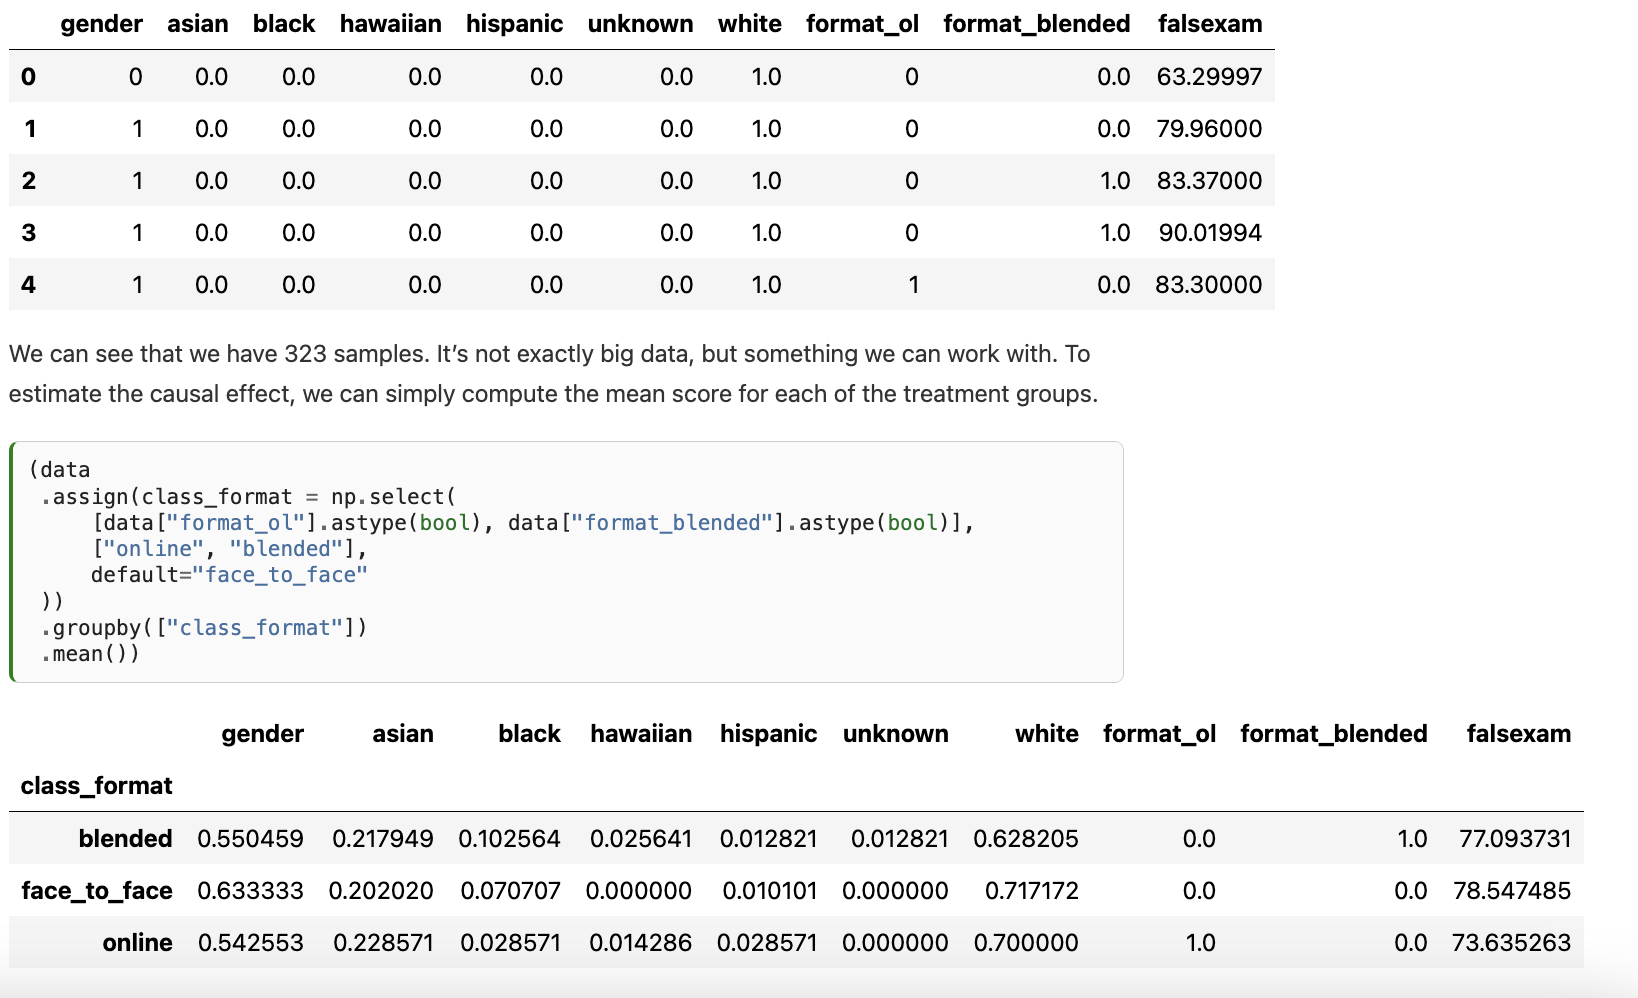
\includegraphics[width=5in]{./imgs/ranex-ex.png}\\\\

In the above example, we can see that by assigning online randomly, we get comparable groups where the outcome before treatment is similar.
The falseexam variable gives an estimate of the outcomes of the 3 groups and the ATE for online students < ATE for offline students.\\\\\\\\
In real world there can be challenges in performing such randomized experiments or randomised controlled trials. Sometimes it's just
unethical to do RCT. For ex - in order to study the effects of smoking during pregnancy, we can't just randomly pick expectant mothers
and ask them to smoke. They are also practially mandatory
for drug trials but still can be challenging to conduct them. They can be also expensive to conduct, hence we do conditional randomization,
to reduce the cost.\\

The assignment that's done during these randomized experiments while can be random, still needs to be informed by informed mechanism about
how the system or world works. In order to understand the direct causal factors, we need to apply the knowledge of system and do the assignment
such that it actually makes the groups comparable. For this, understanding of the assignment mechanism is a must and pivotal to answer 
the causal inference questions.

You can find more information in Chapter 1 of \href{https://matheusfacure.github.io/python-causality-handbook/02-Randomised-Experiments.html}{Causality Handbook}.
\end{document}



